\documentclass[a4paper]{article}
\usepackage[utf8]{inputenc}
\usepackage[a4paper]{geometry}
\geometry{verbose, marginparwidth=15mm, marginparsep=3mm, tmargin=25mm}
\usepackage{tabulary}
\usepackage{enumitem}
\usepackage{graphicx}
\usepackage{float}
\usepackage{multicol}
\usepackage{url}

\title{Redbackup: Projectplan}
\author{
		Fabian Hauser \\
		Raphael Zimmermann
}
\date{\today}


\begin{document}
\maketitle

\section{Project Overview}
The goal of the Study Project is to provide a theoretical description of an append-only, distributed peer-to-peer data storage as well as a working prototype as described in the problem statement \cite{problemstatement}.

The project setting, vision, goals, as well as all other project boundaries, are described in depth in the problem statement \cite{problemstatement}.

\subsection{Components}

For a better overview and to allow us a sophisticated time assessment, we decided to group tasks into categories, i.e. JIRA components. Components represent documents or products which are to be released.

Currently, tasks are separated into following components:

\begin{multicols}{2}
	\begin{itemize}
		\item Final Submission Document
		\item Management
		\item Poster
		\item Presentation
		\item Project Plan
		\item Prototype
	\end{itemize}
\end{multicols}

\section{Project Organization}

The project has a flat structure. All team members have the same strategic rights and duties. Prof. Dr Farhad Mehta is the project advisor and is therefore superior in the organization chart as visible in Figure \ref{fig:organigram}.

\begin{figure}[H]
	\centering
	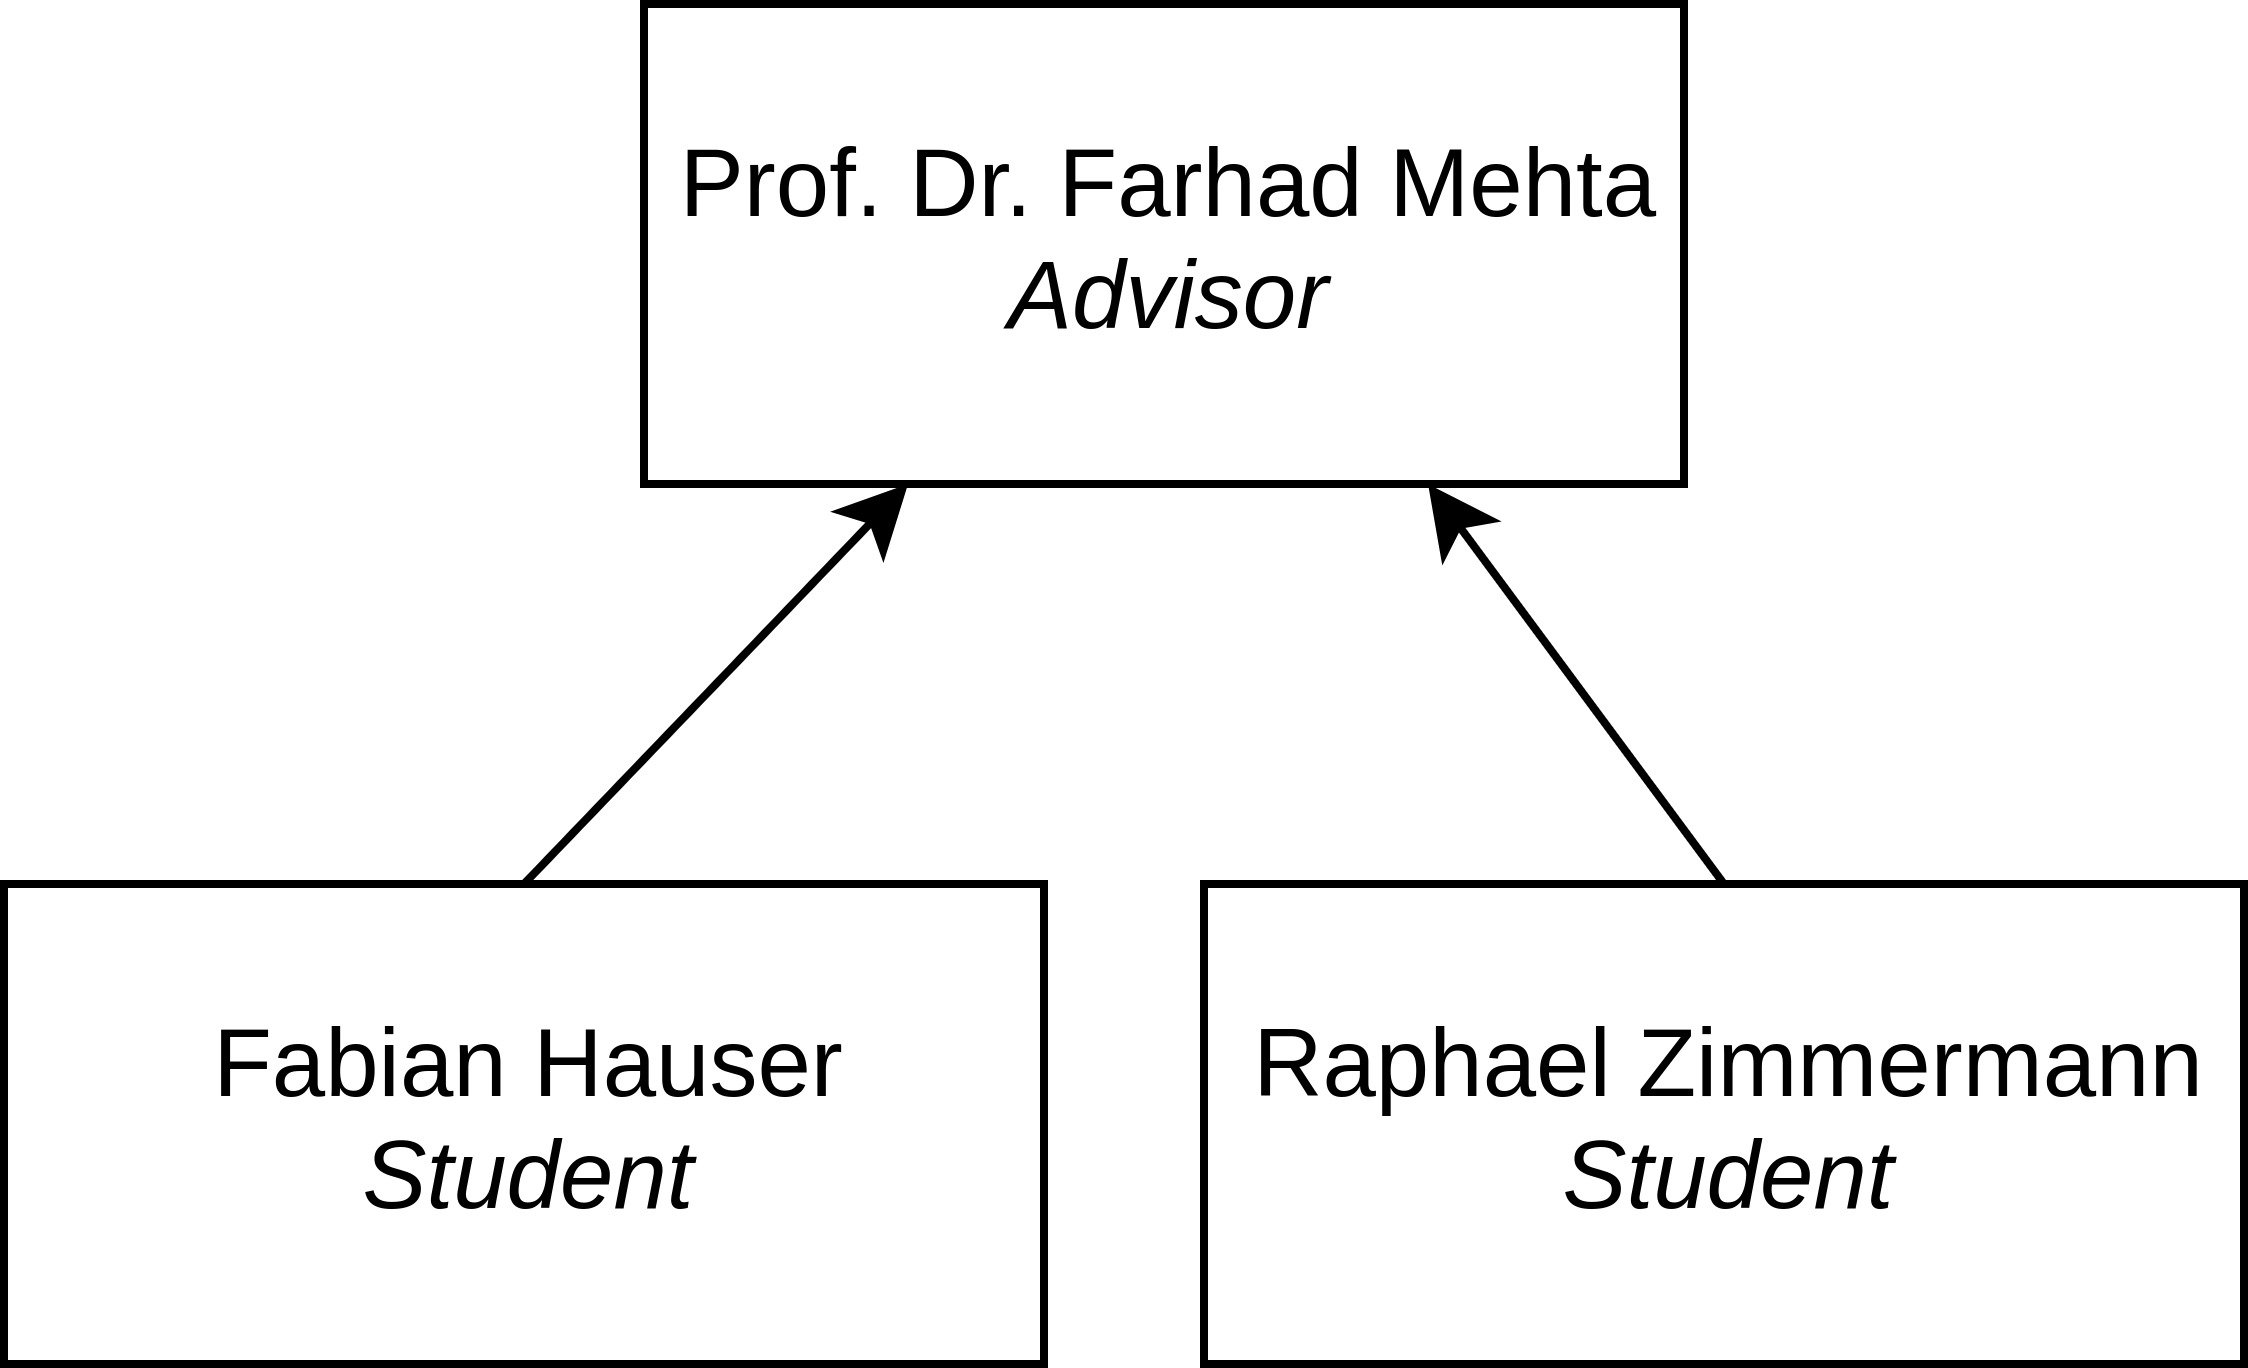
\includegraphics[width=0.5\linewidth]{resources/organigram}
	\caption[Organigram]{Project organization chart}
	\label{fig:organigram}
\end{figure}

\subsection{Roles}

Due to the small team size, most roles are performed by both team members.

\begin{description}
	\item[Raphael Zimmermann] project management, software engineering, quality assurance.
	\item[Fabian Hauser] infrastructure management, software engineering, quality assurance.
\end{description}

\section{Project Workflow}


\section{Risk Management}

\section{Infrastructure}

\section{Quality Measures}
To maintain a high standard of quality, we take the following measures:

\begin{multicols}{2}
	\begin{itemize}
	    \item short sprint reviews
	    \item three extended retrospectives
	    \item code reviews
	    \item automated unit and integration testing
	    \item publish all documentation on the project website using continuous integration/delivery.
	    \item using continuous integration for source code
	\end{itemize}
\end{multicols}

\subsection{Documentation}
The official documents such as the final submission document, the theoretical concept as well as this project plan are written in Latex and published on the project website as pdf documents. All other documents such as meeting minutes are written in markdown and made available in HTML on the website as well.

The sources are in both cases kept under version control in the same repository, which allows us to use the same tools and processes for documentation and code. The continuous integration server builds and publishes the website whenever new changes are pushed to the repository.

\subsection{Project Management}
Because the project plan allows for an iterative process, we use JIRA with its SCRUM-Features (such as sprint creation or boards) for project management.

\subsubsection{Sprint Planning}
Each sprint is mapped to JIRA, which allows the project advisor to trace the project progress. Sprints are represented as boards on which the current state of any issue is easily visible ("To Do", "In Progress", "Review", "Done").


\subsubsection{Definition of Done}
An issue may be closed if \emph{all} of the following conditions are met:

\begin{itemize}
	\item All functionality conforms to the specification. Any deviations must be discussed and decided by the team.
	\item The source code is reasonably documented.
	\item No code is commented out.
	\item No warnings and errors by the compiler or any other quality tool.
	\item A review is performed and accepted in a pull request.
	\item The corresponding branch is merged into the stable branch (e.g. master).
	\item All documents are up to date.
	\item Reasonable unit and integration tests exist and pass.
	\item The complete continuous integration pipeline works.
	\item All time spent on the issue is logged.
\end{itemize}

\subsection{Development}

Since we are in a very early and agile phase we decided to use Github Flow\cite{github-flow}, a straightforward development workflow.

Since the effective technology will be fixed later in the project, concrete coding guidelines, tools, metrics and an error policy will be defined when appropriate.


\subsection{Testing}
All functionality must be testable automatically in continuous integration. Any non-trivial method must be verified with unit tests.

Integration tests verify extended test scenarios.

A minimal performance analysis will be carried out at the end of the project.

\bibliographystyle{abbrv}
\bibliography{refs}

\end{document}
